\documentclass[12pt]{article}
\usepackage[a4paper,margin=1in]{geometry}
\usepackage{amsmath, amssymb}
\usepackage{graphicx}
\usepackage{hyperref}
\usepackage{fancyhdr}

% Header and Footer settings
\pagestyle{fancy}
\fancyhf{}
\rhead{Computer Science Practical File}
\lhead{Class XI}
\cfoot{\thepage}

\begin{document}

\begin{titlepage}
    \includegraphics[width=0.4\textwidth]{logo/lvis-logo.png}
    \centering
    \vspace*{2cm}

    \Huge\textbf{Computer Science Practical File}

    \vspace{1cm}
    \LARGE\textbf{Pranav Verma}

    \vfill

    \Large\textbf{Class: XI Raman}

    \vspace{2cm}

    \Large\textbf{Session: 2024-2025}
\end{titlepage}

\tableofcontents


\section*{Chapter 3: Getting Started with Python \& Chapter 4: Python Programming Fundamentals}
\addcontentsline{toc}{section}{Chapter 3: Getting Started with Python}
\addcontentsline{toc}{section}{Chapter 4: Python Programming Fundamentals}

\subsection*{1. Write a Python program to accept marks in 5 subjects and calculate its mean.}
\begin{verbatim}
a = int(input("Enter the marks in first subject: "))
b = int(input("Enter the marks in second subject: "))
c = int(input("Enter the marks in third subject: "))
d = int(input("Enter the marks in fourth subject: "))
e = int(input("Enter the marks in fifth subject: "))
A = (a + b + c + d + e) / 5
print("Average marks is", A)
\end{verbatim}
\includegraphics[width=\linewidth]{images/1.png}

\subsection*{2. Write a program to enter your name and class.}
\begin{verbatim}
n = input("Enter your name: ")
a = int(input("Enter your age: "))
\end{verbatim}
\includegraphics[width=\linewidth]{images/2.png}

\subsection*{3. Write a program to read details like name, class, and age of a student and then print the details, firstly in the same line and then in separate lines.}
\begin{verbatim}
n = input("Enter your name: ")
c = input("Enter your class: ")
a = input("Enter your age: ")
print(n, c, a)
print(n)
print(c)
print(a)
\end{verbatim}
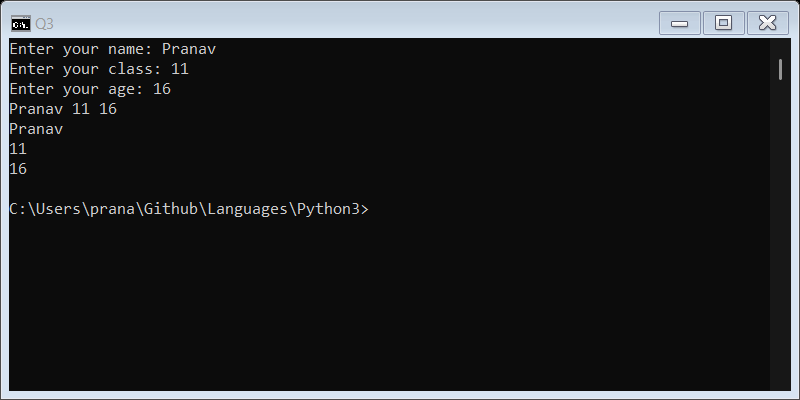
\includegraphics[width=\linewidth]{images/3.png}

\subsection*{4. Celsius to Fahrenheit conversion.}
\begin{verbatim}
c = float(input("Enter the temperature in Celsius: "))
x = (9 * c) / 5
f = 32 + x
print("The temperature in Fahrenheit is", f)
\end{verbatim}
\includegraphics[width=\linewidth]{images/4.png}

\subsection*{5. Write a program to read three numbers in three variables and swap the first two variables with the sums of the first and second, second and third numbers, respectively.}
\begin{verbatim}
a = int(input("Enter the first number: "))
b = int(input("Enter the second number: "))
c = int(input("Enter the third number: "))
a = a + b
b = b + c
print(a, b)
\end{verbatim}
\includegraphics[width=\linewidth]{images/5.png}

\subsection*{6. Write a program to input a number and print the first 5 multiples.}
\begin{verbatim}
n = float(input("Enter the number: "))
print("The first five multiples are", n * 1, n * 2, n * 3, n * 4, "and", n * 5)
\end{verbatim}
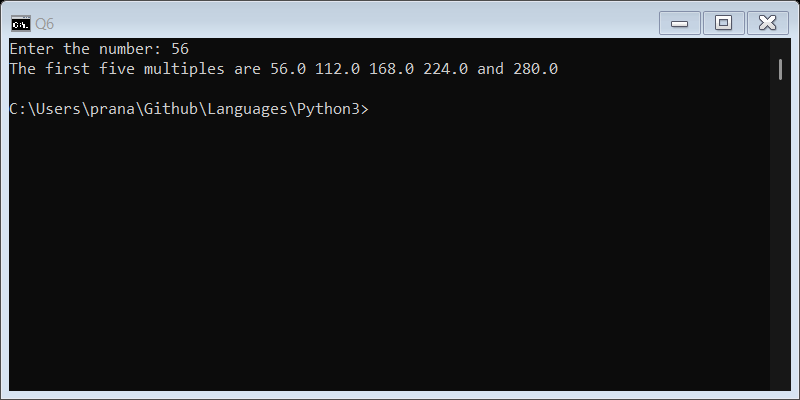
\includegraphics[width=\linewidth]{images/6.png}

\subsection*{7. To calculate the area of a triangle.}
\begin{verbatim}
x = float(input("Enter the base: "))
y = float(input("Enter the height: "))
print("The area is", (x * y) / 2, "units")
\end{verbatim}
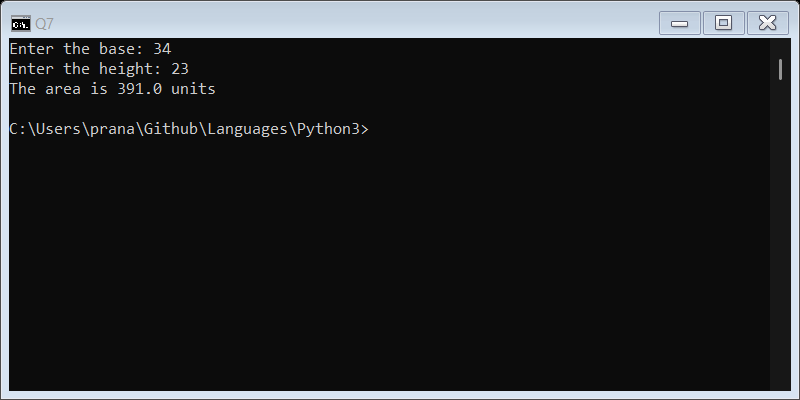
\includegraphics[width=\linewidth]{images/7.png}

\subsection*{8. To calculate the area of a square.}
\begin{verbatim}
x = float(input("Enter the side of the square: "))
print("The area of the square is:", x ** 2)
\end{verbatim}
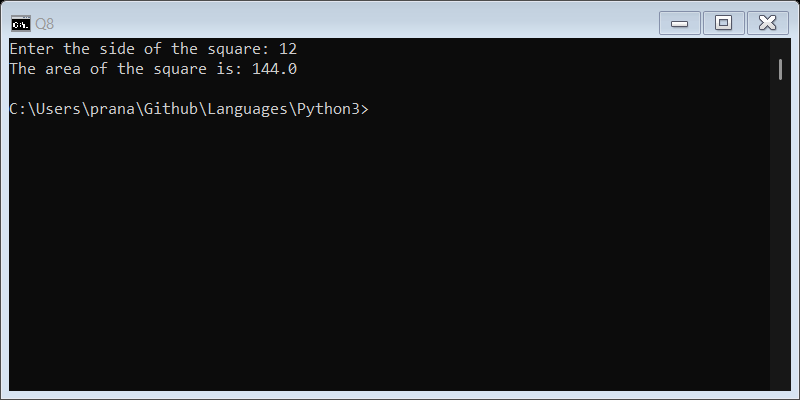
\includegraphics[width=\linewidth]{images/8.png}

\subsection*{9. Take the age from the user and show the year in which the user turns 100 years old.}
\begin{verbatim}
x = int(input("Enter your current age: "))
a = int(input("Enter the current year: "))
y = 100 - x
m = a + y
print("You will turn 100 years old in", m)
\end{verbatim}
\includegraphics[width=\linewidth]{images/9.png}

\subsection*{10. Compound Interest Calculator.}
\begin{verbatim}
P = float(input("Enter the Principle Amount: "))
R = float(input("Enter the Rate of Interest: "))
T = int(input("Enter the Time Period in years: "))
A = P * ((1 + (R / 100)) ** T)
print("The Final Amount is", A)
I = A - P
print("The Interest Amount is", I)
\end{verbatim}
\includegraphics[width=\linewidth]{images/10.png}

\subsection*{11. Write a program to display a name separated by ** sign.}
\begin{verbatim}
N = input("Enter your First Name: ")
S = input("Enter your Surname: ")
print("Name", "Is", N, S, sep='**')
\end{verbatim}
\includegraphics[width=\linewidth]{images/11.png}

\subsection*{12. Write a program to convert money from rupees to paise.}
\begin{verbatim}
R = float(input("Enter the Money in Rs.: "))
p = R * 100
print("Converting Rupees to Paise...")
print("The given money is", p)
\end{verbatim}
\includegraphics[width=\linewidth]{images/12.png}

\subsection*{13. Write a program to print your Name, Class, and Age separated by `/`.}
\begin{verbatim}
x, y, z = input("Enter your Name: "), input("Enter your class: "), input("Enter your age: ")
print(x, y, z, sep="/")
print(x)
print(y)
print(z)
\end{verbatim}
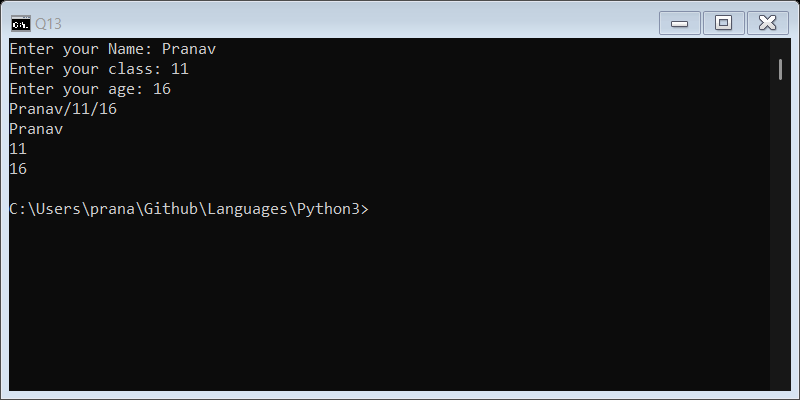
\includegraphics[width=\linewidth]{images/13.png}

\subsection*{14. Write a program to print the Quotient and Remainder of given Dividend and Divisor.}
\begin{verbatim}
D = float(input("Enter the Dividend: "))
d = float(input("Enter the Divisor: "))
print("Calculating the Quotient...")
Q = D // d
print("The Quotient of the given numbers is", Q)
print("Calculating the Remainder...")
R = D % d
print("The Remainder of the given numbers is", R)
\end{verbatim}
\includegraphics[width=\linewidth]{images/14.png}

\subsection*{15. To convert from Celsius to Kelvin.}
\begin{verbatim}
c = float(input("Enter the temperature in Celsius: "))
k = c + 273.15
print("The temperature in Kelvin is", k)
\end{verbatim}
\includegraphics[width=\linewidth]{images/15.png}

\subsection*{16. To find the final velocity of a body.}
\begin{verbatim}
u = float(input("Enter the initial velocity: "))
a = float(input("Enter the acceleration: "))
t = float(input("Enter the time interval: "))
v = u + (a * t)
print("The final velocity is", v)
\end{verbatim}
\includegraphics[width=\linewidth]{images/16.png}

\subsection*{17. To calculate the area of the circle.}
\begin{verbatim}
r = float(input("Enter the radius: "))
a = 3.14 * (r ** 2)
print("The area is", a)
\end{verbatim}
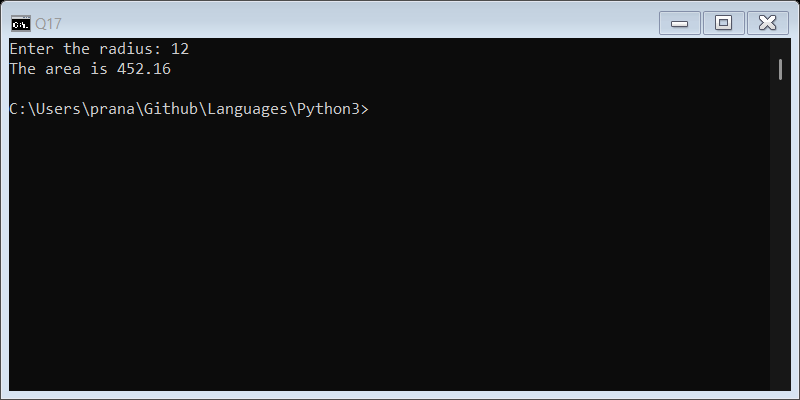
\includegraphics[width=\linewidth]{images/17.png}

\subsection*{18. Hours to minutes converter.}
\begin{verbatim}
h = float(input("Enter the time in hours: "))
m = h * 60
print("The time in minutes is", m)
\end{verbatim}
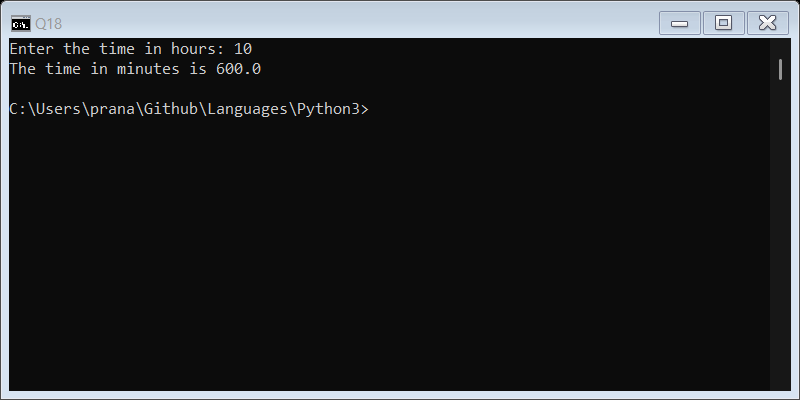
\includegraphics[width=\linewidth]{images/18.png}

\subsection*{19. To calculate the mean of 5 numbers given by the user.}
\begin{verbatim}
a = float(input("Enter the first number: "))
b = float(input("Enter the second number: "))
c = float(input("Enter the third number: "))
d = float(input("Enter the fourth number: "))
e = float(input("Enter the fifth number: "))
m = (a + b + c + d + e) / 5
print("The mean is", m)
\end{verbatim}
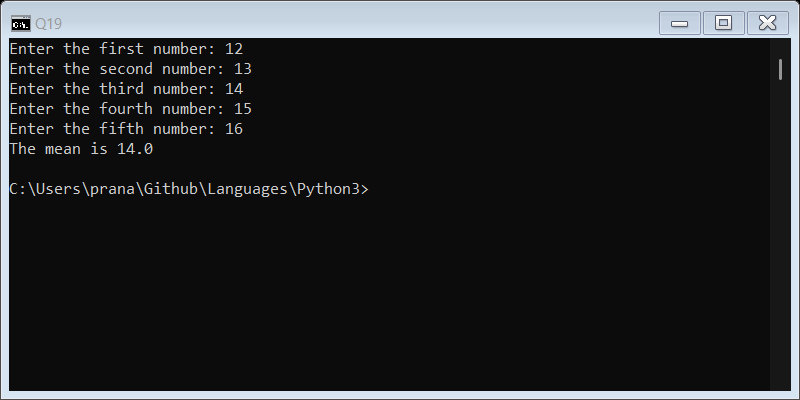
\includegraphics[width=\linewidth]{images/19.png}

\subsection*{20. Meter to kilometer converter.}
\begin{verbatim}
m = float(input("Enter the distance in meters: "))
k = m / 1000
print("Distance in kilometers is", k)
\end{verbatim}
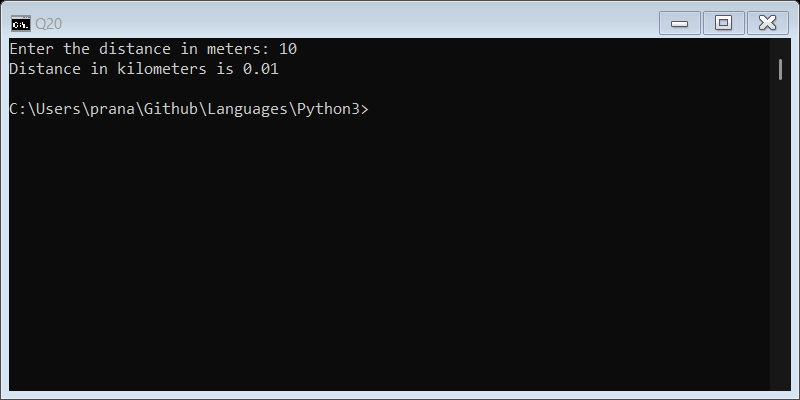
\includegraphics[width=\linewidth]{images/20.png}

\subsection*{21. Litre to millilitre conversion.}
\begin{verbatim}
x = float(input("Enter the amount (in litres): "))
print("The amount in millilitres (ml) is", x * 1000)
\end{verbatim}
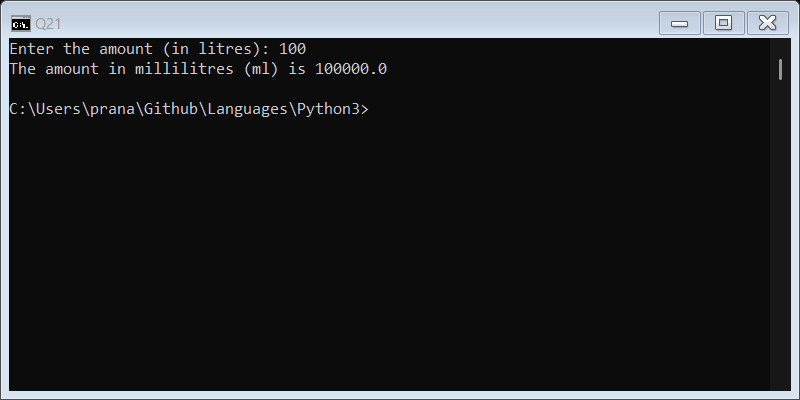
\includegraphics[width=\linewidth]{images/21.png}

\subsection*{22. Time taken by 3 people to do a work.}
\begin{verbatim}
print("Time taken by A to complete the work (in days)")
x = eval(input())
print("Time taken by B to complete the work (in days)")
y = eval(input())
print("Time taken by C to complete the work (in days)")
z = eval(input())
print("Time taken by A, B and C to complete the work together (in days) is")
print((x * y * z) // ((x * y) + (y * z) + (z * x)))
\end{verbatim}
\includegraphics[width=\linewidth]{images/22.png}

\subsection*{23. Calculate the perimeter of a rectangle.}
\begin{verbatim}
l = float(input("Enter the length: "))
b = float(input("Enter the breadth: "))
print("The perimeter is", 2 * (l + b))
\end{verbatim}
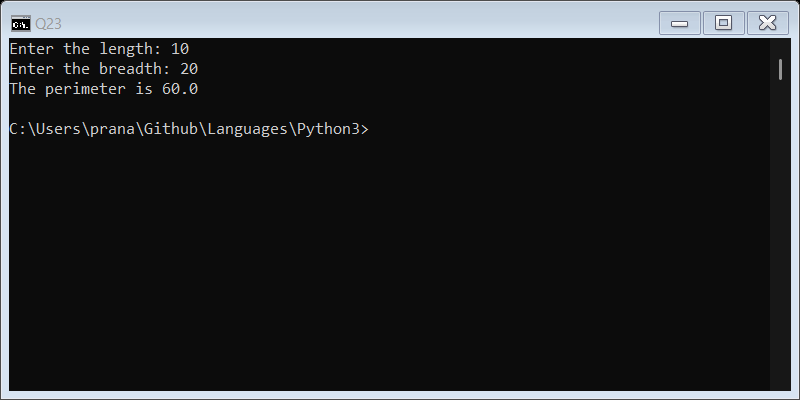
\includegraphics[width=\linewidth]{images/23.png}

\subsection*{24. Write a Python program that accepts cost price and quantity of pencil from the user. Calculate and display total price.}
\begin{verbatim}
c = int(input("Enter the cost price: "))
q = int(input("Enter the quantity: "))
t = c * q
print("Total cost price is", t)
\end{verbatim}
\includegraphics[width=\linewidth]{images/24.png}

\subsection*{25. Write a program to accept time in minutes and convert it into hours and minutes.}
\begin{verbatim}
m = int(input("Enter the time in minutes: "))
h = m // 60
r = m % 60
print("Hours", h)
print("Minutes", r)
\end{verbatim}
\includegraphics[width=\linewidth]{images/25.png}

\subsection*{26. Write a Python program to swap two numbers using a third variable.}
\begin{verbatim}
a = int(input("Enter the value of a: "))
b = int(input("Enter the value of b: "))
print("Before swapping, the values are")
print("Value of a is", a)
print("Value of b is", b)
c = a
a = b
b = c
print("New value of a is", a)
print("New value of b is", b)
\end{verbatim}
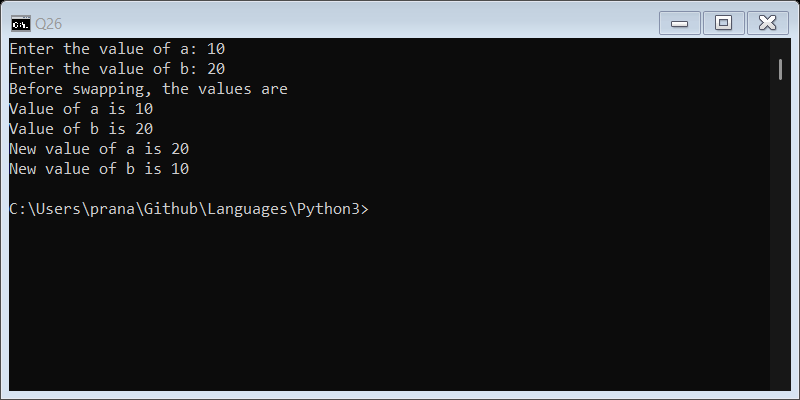
\includegraphics[width=\linewidth]{images/26.png}

\subsection*{27. Write a program to swap two numbers without using a third variable.}
\begin{verbatim}
a = int(input("Enter the value of a: "))
b = int(input("Enter the value of b: "))
print("Before swapping, the values are")
print("Value of a is", a)
print("Value of b is", b)
a = a + b
b = a - b
a = a - b
print("New value of a is", a)
print("New value of b is", b)
\end{verbatim}
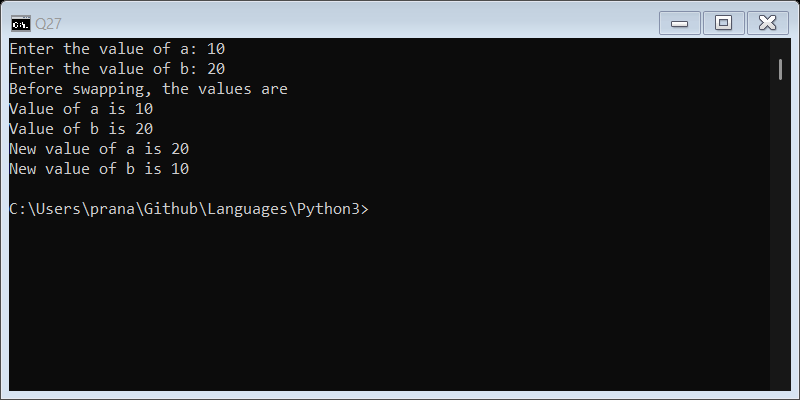
\includegraphics[width=\linewidth]{images/27.png}

\section*{Chapter 5: Conditional and Looping Constructs}
\addcontentsline{toc}{section}{Chapter 5: Conditional and Looping Constructs}

\subsection*{28. A year is a leap year if it is divisible by 4, except that years divisible by 100 are not leap years unless they are also 400. Write a program that asks the user for a year and print whether it is a leap year.}
\begin{verbatim}
y = int(input("Enter the year: "))
if y % 400 == 0 or y % 4 == 0 and y % 100 != 0:
    print("Leap Year")
else:
    print("Not a leap year")
\end{verbatim}
\includegraphics[width=\linewidth]{images/28.png}

\subsection*{29. Write a program to check whether a person is eligible to vote.}
\begin{verbatim}
n = input("Enter your Name: ")
a = int(input("Enter your Age: "))
if a >= 18:
    print(n, "of age", a, "You are Eligible to Vote!!")
else:
    print(n, "of age", a, "You are NOT Eligible to Vote")
\end{verbatim}
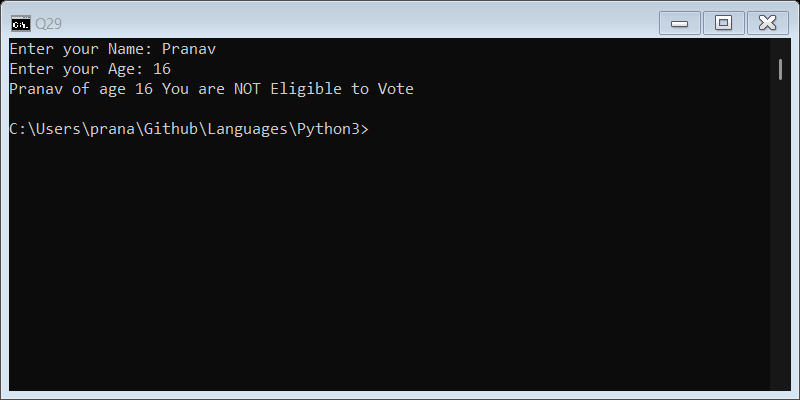
\includegraphics[width=\linewidth]{images/29.png}

\subsection*{30. Check whether a number is odd or even.}
\begin{verbatim}
a = float(input("Enter a Number: "))
x = a % 2
if x == 0:
    print("The Number is Even")
else:
    print("The Number is Odd")
\end{verbatim}
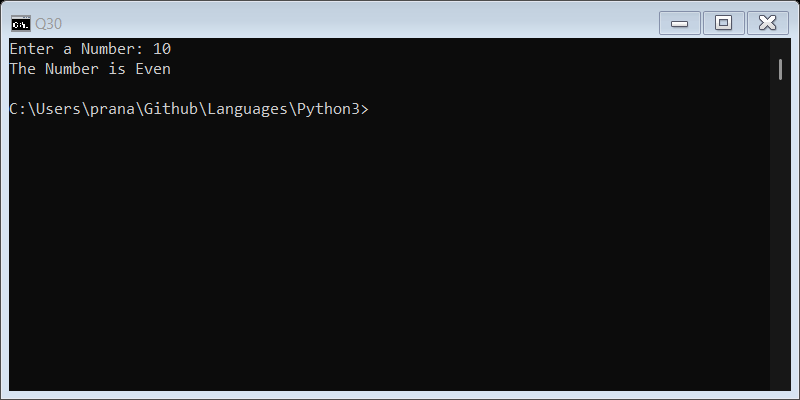
\includegraphics[width=\linewidth]{images/30.png}

\subsection*{31. Write a program to check whether a number between 2 and 30 is Prime or Composite.}
\begin{verbatim}
x = int(input("Enter a Number: "))
y = 0
if 2 <= x <= 30:
    for i in range(2, x):
        if x % i == 0:
            y = 1
            continue
    if y == 0:
        print("The Number is Prime!!")
    else:
        print("The Number is Composite!!")
else:
    print("Enter a Number in range 2 to 30")
\end{verbatim}
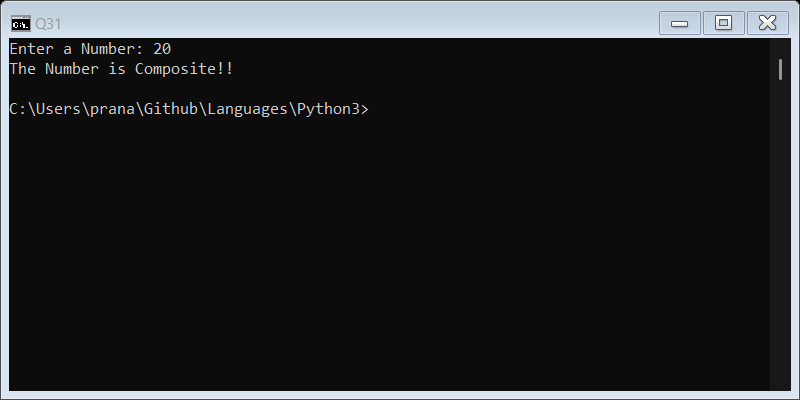
\includegraphics[width=\linewidth]{images/31.png}

\subsection*{32. Write a program to take input from the user and calculate the result of simple problems.}
\begin{verbatim}
a = float(input("Enter the first number: "))
s = input("Enter the Operation to be used: ")
b = float(input("Enter the Second number: "))
if s == '+':
    c = a + b
    print("The addition of", a, "and", b, "is", c)
elif s == '-':
    c = a - b
    print("The difference of", a, "and", b, "is", c)
elif s == '*' or s == "x" or s == "X":
    c = a * b
    print("The product of", a, "and", b, "is", c)
elif s == '/' or s == '÷':
    c = a / b
    print("The division of", a, "and", b, "gives quotient", c)
else:
    print("The given Operator is currently not in the directory")
\end{verbatim}
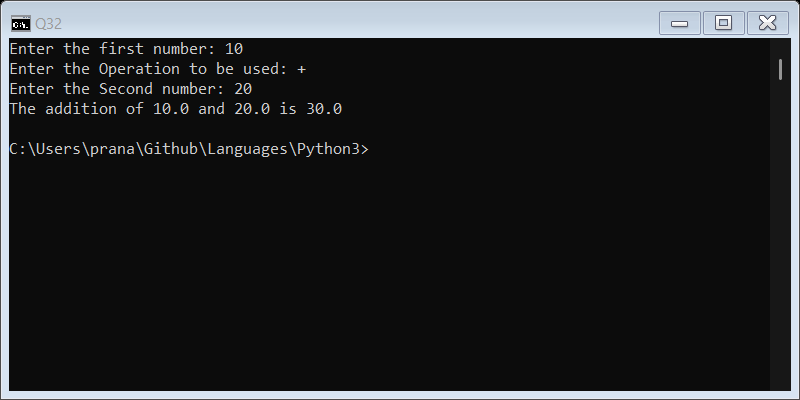
\includegraphics[width=\linewidth]{images/32.png}

\subsection*{33. Write a program to take input of two numbers and find the square of the smaller number and the cube of the greater number.}
\begin{verbatim}
x = float(input("Enter a Number: "))
y = float(input("Enter another Number: "))
if y > x:
    print("The Square of the smaller number, the Cube of the greater number are: -")
    print(x ** 2, y ** 3)
elif x > y:
    print("The Square of the smaller number, the Cube of the greater number are: -")
    print(y ** 2, x ** 3)
elif x == y:
    print("Both Numbers are Equal")
\end{verbatim}
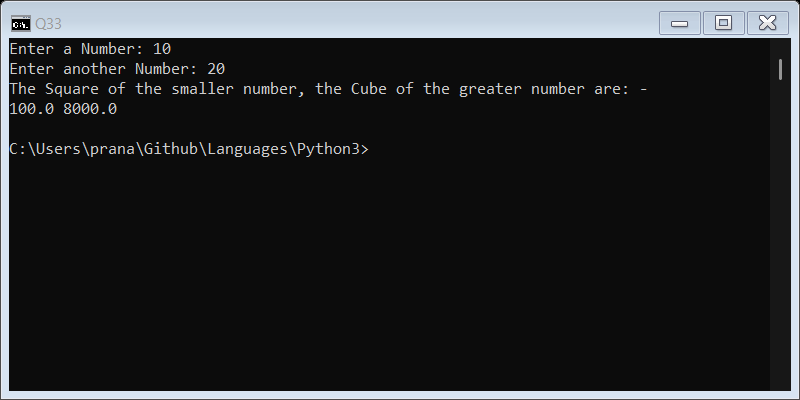
\includegraphics[width=\linewidth]{images/33.png}

\subsection*{34. If the number given by the user is a positive even number, display the 3 successive numbers and if the number is negative and odd, display the 3 preceding numbers.}
\begin{verbatim}
x = float(input("Enter the number: "))
if x > 0:
    if x % 2 == 0:
        print(x + 1, x + 2, x + 3)
    else:
        print("Not a positive even number.")
elif x < 0:
    if x % 2 != 0:
        print(x - 1, x - 2, x - 3)
    else:
        print("Not an odd negative number.")
\end{verbatim}
\includegraphics[width=\linewidth]{images/34.png}

\subsection*{35. Write a program to display the following pattern:}
\begin{verbatim}
for i in range(1, 4):
    for j in range(1, i + 1):
        print(j, end=' ')
    print()
\end{verbatim}
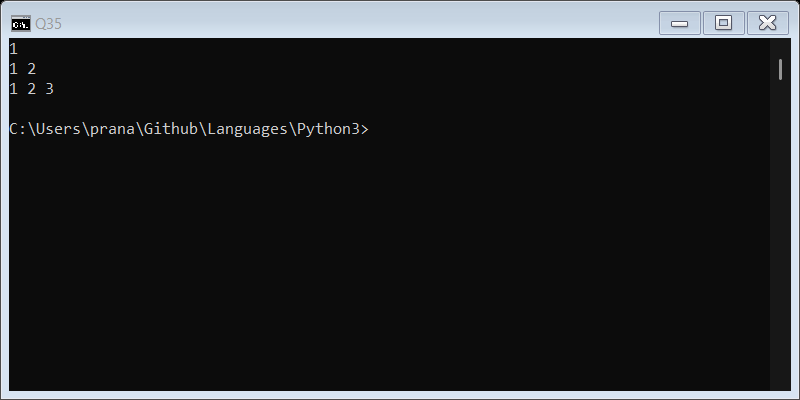
\includegraphics[width=\linewidth]{images/35.png}

\subsection*{36. Write a program to display the following pattern:}
\begin{verbatim}
for i in range(1, 4):
    for j in range(1, i + 1):
        print(i, end=' ')
    print()
\end{verbatim}
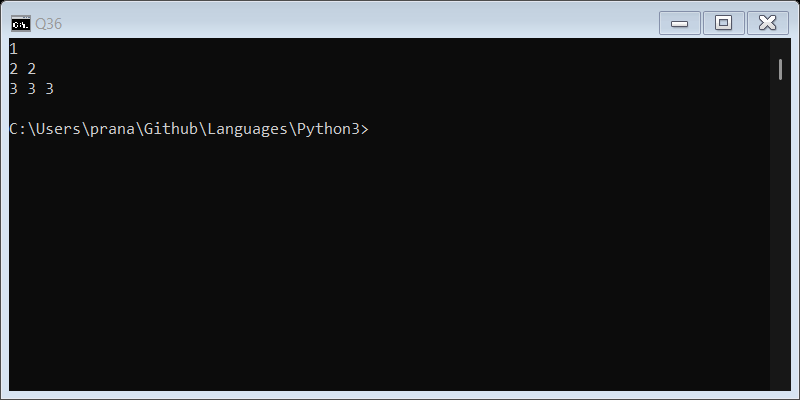
\includegraphics[width=\linewidth]{images/36.png}

\subsection*{37. Write a program to display the following pattern:}
\begin{verbatim}
c = 0
for i in range(1, 5):
    for j in range(1, i + 1):
        c = c + 1
        print(c, end=' ')
    print()
\end{verbatim}
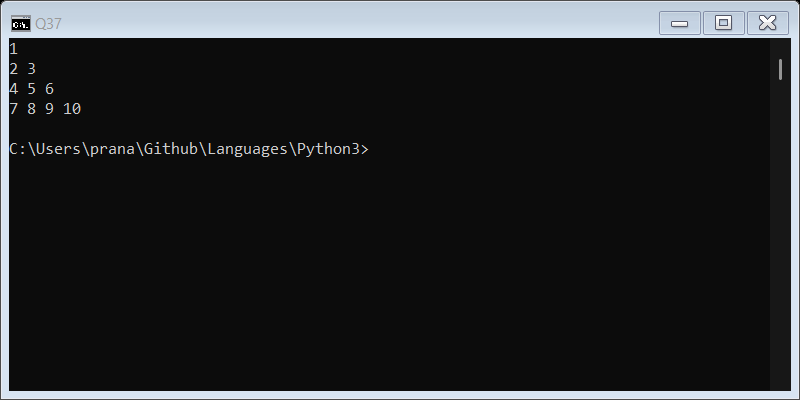
\includegraphics[width=\linewidth]{images/37.png}

\subsection*{38. Write a program to display the following pattern:}
\begin{verbatim}
for i in range(4, 0, -1):
    for j in range(i, 0, -1):
        print(j, end=' ')
    print()
\end{verbatim}
\includegraphics[width=\linewidth]{images/38.png}

\subsection*{39. Write a Python program to sum two integers. However, if the sum is between 15 to 20 it will return 20.}
\begin{verbatim}
a = int(input("Enter the first number: "))
b = int(input("Enter the second number: "))
m = a + b
if m > 15 and m < 20:
    print("20")
else:
    print(m)
\end{verbatim}
\includegraphics[width=\linewidth]{images/39.png}

\subsection*{40. Check whether a triangle is equilateral, scalene, or isosceles.}
\begin{verbatim}
a = float(input("Enter the length of the first side: "))
b = float(input("Enter the length of the second side: "))
c = float(input("Enter the length of the third side: "))
if a == b == c:
    print("Equilateral triangle")
elif a == b and a != c:
    print("Isosceles triangle")
elif b == c and c != a:
    print("Isosceles triangle")
elif a == c and a != b:
    print("Isosceles triangle")
elif a != b and b != c and a != c:
    print("Scalene triangle")
\end{verbatim}
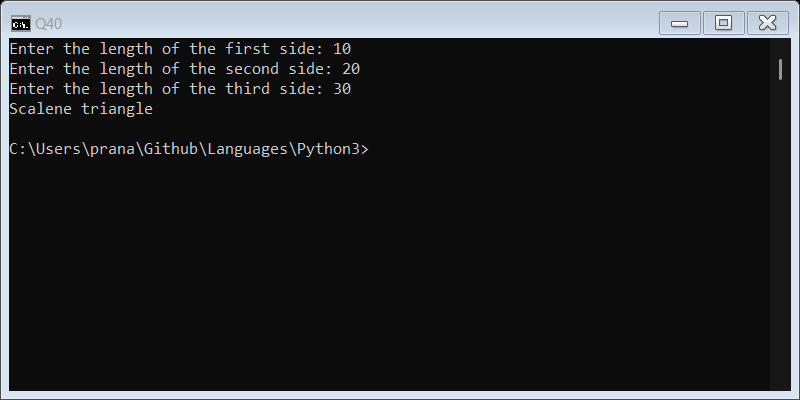
\includegraphics[width=\linewidth]{images/40.png}

\subsection*{41. Display the factorial of a number.}
\begin{verbatim}
x = int(input("Enter a positive integer: "))
c = 1
for i in range(1, x + 1):
    c = c * i
print("Its factorial is", c)
\end{verbatim}
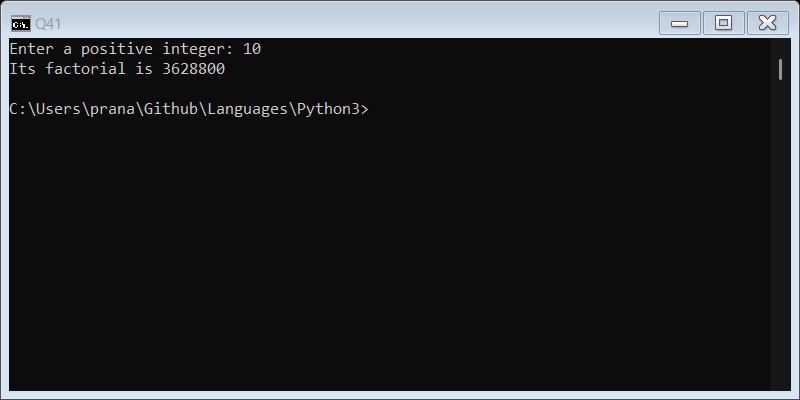
\includegraphics[width=\linewidth]{images/41.png}

\subsection*{42. Print the first 10 even numbers.}
\begin{verbatim}
for i in range(1, 21):
    if i % 2 == 0:
        print(i)
\end{verbatim}
\includegraphics[width=\linewidth]{images/42.png}

\subsection*{43. Write a code to check whether a number is composite or not.}
\begin{verbatim}
x = int(input("Enter an integer: "))
for i in range(2, x):
    if x % i == 0:
        print("Composite number")
        break
else:
    print("Prime")
\end{verbatim}
\includegraphics[width=\linewidth]{images/43.png}

\subsection*{44. Write a code to check whether a number is prime or not.}
\begin{verbatim}
x = int(input("Enter an integer: "))
if x < 2:
    print("Not prime")
else:
    for i in range(2, int(x**0.5) + 1):
        if x % i == 0:
            print("Not prime")
            break
    else:
        print("Prime")    
\end{verbatim}
\includegraphics[width=\linewidth]{images/44.png}

\subsection*{45. Take a month from the user and display the number of days.}
\begin{verbatim}
m = input("Enter the month: ")
n = m.lower()
x = "january, march, may, july, august, october, december"
y = "february"
z = "april, june, september, november"
if n in x:
    print("31 days")
elif n == y:
    print("28 or 29 days")
else:
    print("30 days")
\end{verbatim}
\includegraphics[width=\linewidth]{images/45.png}

\subsection*{46. Write a program that reads two integers representing a month and day and prints the season for that month and day.}
\begin{verbatim}
x = input("Enter the month: ")
d = int(input("Enter the date: "))
y = x.lower()
s = "april, may, june"
m = "july, august, september"
a = "october"
w = "november, december, january, february"
sp = "march"
if y in s:
    print("Summer season")
elif y in m:
    print("Monsoon season")
elif y in w:
    print("Winter season")
elif y in a:
    print("Autumn season")
elif y in sp:
    print("Spring season")
\end{verbatim}
\includegraphics[width=\linewidth]{images/46.png}

\subsection*{47. Write a program to display the astrological sign for a given date of birth.}
\begin{verbatim}
x = int(input("Enter your birth date (for example: Enter 25 for 25th October): "))
y = input("Enter your birth month: ")
z = y.lower()
if x >= 21 and x < 32 and z == "march":
    print("Aries")
elif x < 21 and z == "april":
    print("Aries")
elif x >= 21 and x < 32 and z == "april":
    print("Taurus")
elif x < 21 and z == "may":
    print("Taurus")
elif x >= 21 and x < 32 and z == "may":
    print("Gemini")
elif x < 21 and z == "june":
    print("Gemini")
elif x >= 21 and x < 32 and z == "june":
    print("Cancer")
elif x < 21 and z == "july":
    print("Cancer")
elif x >= 21 and x < 32 and z == "july":
    print("Leo")
elif x < 21 and z == "august":
    print("Leo")
elif x >= 21 and x < 32 and z == "august":
    print("Virgo")
elif x < 21 and z == "september":
    print("Virgo")
elif x >= 21 and x < 32 and z == "september":
    print("Libra")
elif x < 21 and z == "october":
    print("Libra")
elif x >= 21 and x < 32 and z == "october":
    print("Scorpio")
elif x < 21 and z == "november":
    print("Scorpio")
elif x >= 21 and x < 32 and z == "november":
    print("Sagittarius")
elif x < 21 and z == "december":
    print("Sagittarius")
elif x >= 21 and x < 32 and z == "december":
    print("Capricorn")
elif x < 21 and z == "january":
    print("Capricorn")
elif x >= 21 and x < 32 and z == "january":
    print("Aquarius")
elif x < 21 and z == "february":
    print("Aquarius")
elif x >= 21 and x < 32 and z == "february":
    print("Pisces")
elif x < 21 and z == "march":
    print("Pisces")
\end{verbatim}
\includegraphics[width=\linewidth]{images/47.png}

\subsection*{48. Pyramid star.}
\begin{verbatim}
n = int(input("Enter the number of lines: "))
for i in range(1, n + 1):
    for j in range(1, i + 1):
        print("*", end=' ')
    print()
\end{verbatim}
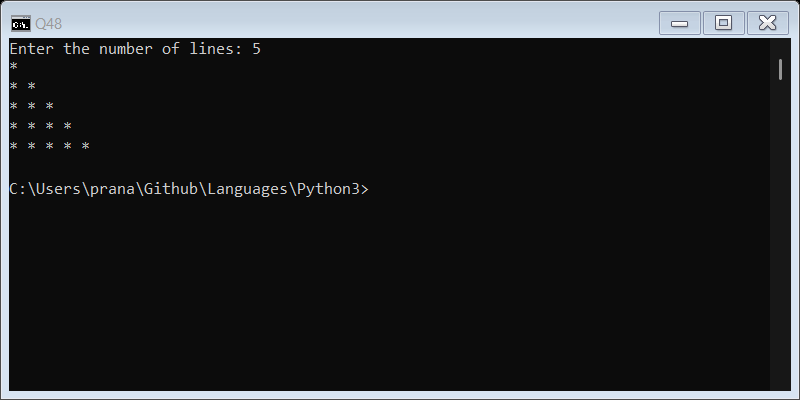
\includegraphics[width=\linewidth]{images/48.png}

\subsection*{49. Display every letter of your name in separate lines.}
\begin{verbatim}
n = input("Enter your name: ")
for i in n:
    print(i)
\end{verbatim}
\includegraphics[width=\linewidth]{images/49.png}

\subsection*{50. Write a program to get the next day of a given date.}
\begin{verbatim}
a = int(input("Enter the date: "))
b = int(input("Enter the month: "))
c = int(input("Enter the year: "))
if a >= 1 and a < 31:
    if b == 1 or b == 3 or b == 5 or b == 7 or b == 8 or b == 10 or b == 12:
        a = a + 1
        print(a, b, c)
    elif a == 31:
        if b == 1 or b == 3 or b == 5 or b == 7 or b == 8 or b == 10:
            b = b + 1
            print(1, b, c)
        elif a == 31 and b == 12:
            print(1, 1, c + 1)
    elif a >= 1 and a < 30:
        if b == 2 or b == 4 or b == 6 or b == 9 or b == 11:
            print(a + 1, b, c)
\end{verbatim}
\includegraphics[width=\linewidth]{images/50.png}

\subsection*{51. Write a program to input three numbers and check whether they are equal or not. If they are unequal then display the greatest and smallest numbers, if they are equal, then display "numbers are equal".}
\begin{verbatim}
a = float(input("Enter the first number: "))
b = float(input("Enter the second number: "))
c = float(input("Enter the third number: "))
if a == b == c:
    print("Equal")
elif a > b and b > c:
    print("Greatest:", a, "Smallest:", c)
elif b > a and a > c:
    print("Greatest:", b, "Smallest:", c)
elif c > a and a > b:
    print("Greatest:", c, "Smallest:", b)
elif a > c and c > b:
    print("Greatest:", a, "Smallest:", b)
elif b > c and c > a:
    print("Greatest:", b, "Smallest:", a)
elif c > b and b > a:
    print("Greatest:", c, "Smallest:", a)
elif a > b and b == c:
    print("Greatest:", a, "Smallest:", c)
elif b > a and a == c:
    print("Greatest:", b, "Smallest:", c)
elif c > b and a == b:
    print("Greatest:", c, "Smallest:", b)
elif a < b and b == c:
    print("Greatest:", b, "Smallest:", a)
elif b < a and a == c:
    print("Greatest:", a, "Smallest:", b)
elif c < b and a == b:
    print("Greatest:", b, "Smallest:", c)
\end{verbatim}
\includegraphics[width=\linewidth]{images/51.png}

\subsection*{52. A special two-digit number is such that when the sum of its digits is added to the product of the digits, the result will be the same as the original number.}
\begin{verbatim}
x = int(input("Enter the two-digit number: "))
y = x // 10
z = x % 10
s = y + z
p = y * z
if s + p == x:
    print("It is a special number")
else:
    print("It is not a special number")
\end{verbatim}
\includegraphics[width=\linewidth]{images/52.png}

\subsection*{53. Income Tax Calculator.}
\begin{verbatim}
x = input("Enter your name: ")
a = int(input("Enter your age: "))
n = float(input("Enter your income: "))
if a > 60:
    print("Wrong Category")
elif a <= 60:
    if n <= 500000:
        print("NIL")
    elif n > 500000 and n <= 750000:
        t = (n - 500000) * (0.1)
        print("Name:", x, "Age:", a, "Income tax:", t)
    elif n > 750000 and n <= 1000000:
        t = ((n - 750000) * (0.2)) + 30000
        print("Name:", x, "Age:", a, "Income tax:", t)
    elif n > 1000000:
        t = ((n - 1000000) * (0.3)) + 90000
        print("Name:", x, "Age:", a, "Income tax:", t)
\end{verbatim}
\includegraphics[width=\linewidth]{images/53.png}

\subsection*{54. Write a program to display the sum of the given series: Sum = 1 + (1 + 2) + (1 + 2 + 3) + (1 + 2 + 3 + ... n).}
\begin{verbatim}
n = int(input("Enter the value of n: "))
c = 0
s = 0
d = 0
for i in range(1, n + 1):
    c = c + 1
    s = s + c
    d = d + s
print(d)
\end{verbatim}
\includegraphics[width=\linewidth]{images/54.png}

\subsection*{55. Write a program to display the series: 1 - x\^1 / 2! + x\^2 / 3! - x\^3 / 4! + x\^5 / 5! ... x\^n / (n + 1)!.}
\begin{verbatim}
n = int(input("Enter the value of n: "))
x = int(input("Enter the value of x: "))
f = 1
t = 0
s = 0
for i in range(1, n + 2):
    f = f * i
    for j in range(0, i):
        if j % 2 != 0:
            t = -((x * j) / f)
        elif j % 2 == 0:
            t = (x * j) / f
        s = s + t
print(s)
\end{verbatim}
\includegraphics[width=\linewidth]{images/55.png}

\section*{Chapter 6: Strings in Python}
\addcontentsline{toc}{section}{Chapter 6: Strings in Python}

\subsection*{56. Given a string, if its length is at least 3, add 'ing' to its end. Unless it already ends in 'ing', in which case add 'ly' instead. If the string length is less than 3, leave it unchanged. Return the resulting string.}
\begin{verbatim}
x = input("Enter the string: ")
if len(x) >= 3:
    if x.endswith("ing"):
        x = x + "ly"
    else:
        x = x + "ing"
print(x)
\end{verbatim}
\includegraphics[width=\linewidth]{images/56.png}

\subsection*{57. Given a string s, return a string made of the first 2 and the last 2 chars of the original string, so 'spring' yields 'spng'. However, if the string length is less than 2, return instead the empty string.}
\begin{verbatim}
x = input("Enter the string: ")
if len(x) >= 2:
    x = x[0:2] + x[-1:-3:-1]
    print(x)
else:
    print(x)
\end{verbatim}
\includegraphics[width=\linewidth]{images/57.png}

\subsection*{58. Given a string s, return a string where all occurrences of its first char have been changed to *, except do not change the first char itself. e.g. 'babble' yields 'ba**le'.}
\begin{verbatim}
x = input("Enter the string: ")
y = x[1:]
for i in y:
    if i == x[0]:
        y = y.replace(i, "*")
x = x[0] + y
print(x)
\end{verbatim}
\includegraphics[width=\linewidth]{images/58.png}

\subsection*{59. Given strings a and b, return a single string with a and b separated by a space '<a> <b>', except swap the first 2 chars of each string. e.g. 'mix', 'pod' -> 'pox mid', 'dog', 'dinner' -> 'dig donner'. Assume a and b are length 2 or more.}
\begin{verbatim}
x = input("Enter the string: ")
y = input("Enter another string: ")
x = y[0:2] + x[2:]
y = x[0:2] + y[2:]
print(x, y)
\end{verbatim}
\includegraphics[width=\linewidth]{images/59.png}

\subsection*{60. Given a string, find the first appearance of the substring 'not' and 'bad'. If the 'bad' follows the 'not', replace the whole 'not'...'bad' substring with 'good'. Return the resulting string. So 'This dinner is not that bad!' yields: This dinner is good!}
\begin{verbatim}
x = input("Enter the string: ")
y = x.find("not")
z = x.find("bad")
s = 0
if z > y:
    s = x[y:z + 3]
    x = x.replace(s, "good")
print(x)
\end{verbatim}
\includegraphics[width=\linewidth]{images/60.png}

\subsection*{61. Consider dividing a string into two halves. If the length is even, the front and back halves are the same length. If the length is odd, we'll say that the extra char goes in the front half. e.g. 'abcde', the front half is 'abc', the back half 'de'. Given 2 strings, a and b, return a string of the form - a-front + b-front + a-back + b-back.}
\begin{verbatim}
a = input("Enter the first string: ")
b = input("Enter the second string: ")
m = len(a)
if m % 2 != 0:
    n = (m - 1) // 2
else:
    n = m // 2
afront = a[0:n + 1]
aback = a[n + 1:]
x = len(b)
if x % 2 != 0:
    y = (x - 1) // 2
else:
    y = x // 2
bfront = b[0:n + 1]
bback = b[n + 1:]
c = afront + bfront + aback + bback
print(c)
\end{verbatim}
\includegraphics[width=\linewidth]{images/61.png}

\subsection*{62. Python Program to Replace all Occurrences of 'a' with \$ in a String.}
\begin{verbatim}
x = input("Enter the string: ")
y = x.replace("a", "\$")
print(y)
\end{verbatim}
\includegraphics[width=\linewidth]{images/62.png}

\subsection*{63. Python Program to Remove the nth Index Character from a Non-Empty String.}
\begin{verbatim}
x = input("Enter the string: ")
n = int(input("Enter the index: "))
x = x[0:n] + x[n + 1:]
print(x)
\end{verbatim}
\includegraphics[width=\linewidth]{images/63.png}

\subsection*{64. Python Program to Detect if Two Strings are Anagrams.}
\begin{verbatim}
x = input("Enter the string: ")
y = input("Enter another string: ")
if len(x) == len(y):
    for i in x:
        if i not in y:
            print("Not an anagram")
            break
    else:
        print("Anagram")
else:
    print("Not anagrams")
\end{verbatim}
\includegraphics[width=\linewidth]{images/64.png}

\subsection*{65. Python Program to Form a New String where the First Character and the Last Character have been Exchanged.}
\begin{verbatim}
x = input("Enter the string: ")
y = len(x)
x = x[-1] + x[1:y] + x[0]
print(x)
\end{verbatim}
\includegraphics[width=\linewidth]{images/65.png}

\subsection*{66. Python Program to Count the Number of Vowels in a String.}
\begin{verbatim}
x = input("Enter the string: ")
x = x.lower()
s = 'aeiou'
c = 0
for i in x:
    if i in s:
        c = c + 1
print(c)
\end{verbatim}
\includegraphics[width=\linewidth]{images/66.png}

\subsection*{67. Python Program to Take in a String and Replace Every Blank Space with Hyphen.}
\begin{verbatim}
x = input("Enter the string: ")
x = x.replace(" ", "-")
print(x)
\end{verbatim}
\includegraphics[width=\linewidth]{images/67.png}

\subsection*{68. Python Program to Calculate the Length of a String Without Using a Library Function.}
\begin{verbatim}
x = input("Enter the string: ")
c = 0
for i in x:
    c = c + 1
print(c)
\end{verbatim}
\includegraphics[width=\linewidth]{images/68.png}

\subsection*{69. Python Program to Calculate the Number of Words and the Number of Characters Present in a String.}
\begin{verbatim}
x = input("Enter the string: ")
c = 0
s = "0123456789"
d = 0
for i in x:
    if i.isalpha() == True:
        c = c + 1
for j in x:
    if j in s:
        d = d + 1
print(c, "letters")
print(c + d, "characters")
\end{verbatim}
\includegraphics[width=\linewidth]{images/69.png}

\subsection*{70. Python Program to Take in Two Strings and Display the Larger String without Using Built-in Functions.}
\begin{verbatim}
x = input("Enter the string: ")
y = input("Enter another string: ")
c = 0
d = 0
for i in x:
    c = c + 1
for j in y:
    d = d + 1
if d > c:
    print(y, "is the larger string")
elif c > d:
    print(x, "is the larger string")
\end{verbatim}
\includegraphics[width=\linewidth]{images/70.png}

\subsection*{71. Python Program to Count Number of Lowercase Characters in a String.}
\begin{verbatim}
x = input("Enter the string: ")
c = 0
for i in x:
    if i.islower() == True:
        c = c + 1
print(c)
\end{verbatim}
\includegraphics[width=\linewidth]{images/71.png}

\subsection*{72. Python Program to Check if a String is a Palindrome or Not.}
\begin{verbatim}
x = input("Enter the string: ")
y = x[-1::-1]
if x == y:
    print("It is a palindrome")
else:
    print("Not a palindrome")
\end{verbatim}
\includegraphics[width=\linewidth]{images/72.png}

\subsection*{73. Python Program to Calculate the Number of Upper Case Letters and Lower Case Letters in a String.}
\begin{verbatim}
x = input("Enter the string: ")
u = 0
l = 0
for i in x:
    if i.islower() == True:
        l = l + 1
    else:
        u = u + 1
print(l, "lowercase characters", u, "uppercase characters")
\end{verbatim}
\includegraphics[width=\linewidth]{images/73.png}

\subsection*{74. Python Program to Check if a String is a Pangram or Not.}
\begin{verbatim}
x = input("Enter a string: ")
s = "abcdefghijklmnopqrstuvwxyz"
for i in s:
    if i not in x:
        print("Not a pangram")
        break
else:
    print("It is a pangram")
\end{verbatim}
\includegraphics[width=\linewidth]{images/74.png}

\subsection*{75. Python Program to Calculate the Number of Digits and Letters in a String.}
\begin{verbatim}
x = input("Enter the string: ")
c = 0
s = "0123456789"
d = 0
for i in x:
    if i.isalpha() == True:
        c = c + 1
for j in x:
    if j in s:
        d = d + 1
print(c, "letters")
print(d, "digits")
\end{verbatim}
\includegraphics[width=\linewidth]{images/75.png}

\subsection*{76. Python Program to Form a New String Made of the First 2 and Last 2 Characters From a Given String.}
\begin{verbatim}
x = input("Enter the string: ")
y = x[0:2] + x[-1:-3:-1]
print(y)
\end{verbatim}
\includegraphics[width=\linewidth]{images/76.png}

\section*{Chapter 7: Lists}
\addcontentsline{toc}{section}{Chapter 7: Lists}

\subsection*{77. Write a program to read a list of elements. Modify this list so that it does not contain any duplicate elements, i.e., all elements occurring multiple times in the list should appear only once.}
\begin{verbatim}
x = eval(input("Enter the list: "))
y = []
for i in range(len(x)):
    m = x.index(x[i])
    if i == m:
        y.insert(i, x[i])
print(y)
\end{verbatim}
\includegraphics[width=\linewidth]{images/77.png}

\subsection*{78. Write a program to create a list of elements. Input an element from the user that has to be inserted in the list. Also input the position at which it is to be inserted.}
\begin{verbatim}
x = eval(input("Enter the list: "))
a = input("Enter the element to be inserted: ")
n = int(input("Enter the position at which it is to be inserted: "))
x.insert(n - 1, a)
print(x)
\end{verbatim}
\includegraphics[width=\linewidth]{images/78.png}

\subsection*{79. Write a program which asks for the position of the element to be deleted from the list and delete the desired element at the desired position.}
\begin{verbatim}
x = eval(input("Enter the list: "))
n = int(input("Enter the position of the element that is to be removed: "))
x.pop(n - 1)
print(x)
\end{verbatim}
\includegraphics[width=\linewidth]{images/79.png}

\subsection*{80. Write a program which asks for the value of the element to be deleted from the list and delete the desired element at the desired position.}
\begin{verbatim}
x = eval(input("Enter the list: "))
a = int(input("Enter the position of the element to be removed: "))
if 0 <= a < len(x):
    x.pop(a)
    print("Updated list:", x)
else:
    print("Invalid position. Please enter a valid index.")
\end{verbatim}
\includegraphics[width=\linewidth]{images/80.png}

\subsection*{81. Write a program that takes an array S as an argument and all the odd values and display the sum.}
\begin{verbatim}
s = eval(input("Enter the list in square brackets: "))
t = 0
for i in range(len(s)):
    if i % 2 == 0:
        t = t + s[i]
print(t)
\end{verbatim}
\includegraphics[width=\linewidth]{images/81.png}

\subsection*{82. Write a program to calculate the mean of a given list of numbers.}
\begin{verbatim}
x = eval(input("Enter the list: "))
s = 0
for i in x:
    s = s + i
s = s / len(x)
print(s)
\end{verbatim}
\includegraphics[width=\linewidth]{images/82.png}

\subsection*{83. Write a program to delete all duplicate elements in a list.}
\begin{verbatim}
l = eval(input("Enter the list: "))
for i in range(len(l) - 1, 0, -1):
    if l.count(l[i]) > 1:
        l.remove(l[i])
print(l)
\end{verbatim}
\includegraphics[width=\linewidth]{images/83.png}

\subsection*{84. Write a program to calculate the minimum element of a given list.}
\begin{verbatim}
l = eval(input("Enter the list: "))
s = []
num = []
    
for i in l:
    if isinstance(i, str): 
        s.append(i)
    elif isinstance(i, (int, float)):
        num.append(i)
    
if s:
    print("Minimum string:", min(s))
else:
    print("No strings in the list.")
    
if num:
    print("Minimum number:", min(num))
else:
    print("No numbers in the list.")    
\end{verbatim}
\includegraphics[width=\linewidth]{images/84.png}

\subsection*{85. Write a code to calculate and display the total marks and percentage of a student from the given list storing marks of a student.}
\begin{verbatim}
l = eval(input("Enter the list: "))
total = 0
perc = 0
for i in l:
    total += i
perc = (total / len(l))
print("Marks:", total, "Percentage:", perc)
\end{verbatim}
\includegraphics[width=\linewidth]{images/85.png}

\subsection*{86. Write a program to multiply an element by 2 if it is at an odd index for a given list storing marks of a student.}
\begin{verbatim}
l = eval(input("Enter the list: "))
for i in range(len(l)):
    if i % 2 != 0:
        l[i] = l[i] * 2
print(l)
\end{verbatim}
\includegraphics[width=\linewidth]{images/86.png}

\subsection*{87. Write a program to multiply an element by 2 if it is at an odd index for a given list containing both numbers and strings.}
\begin{verbatim}
l = eval(input("Enter the list: "))
for i in range(len(l)):
    if i % 2 != 0:
        l[i] = l[i] * 2
print(l)
\end{verbatim}
\includegraphics[width=\linewidth]{images/87.png}

\subsection*{88. Write a program to calculate the frequency of an element in a given list.}
\begin{verbatim}
l = eval(input("Enter the list: "))
x = input("Enter the element: ")
print("Frequency of", x, "is", l.count(x))
\end{verbatim}
\includegraphics[width=\linewidth]{images/88.png}
\subsection*{89. Write a program to find the second largest number in a list.}
\begin{verbatim}
l = eval(input("Enter the list: "))
l.sort()
print("The second largest number is:", l[-2])
\end{verbatim}
\includegraphics[width=\linewidth]{images/89.png}

\subsection*{90. Write a program to find the common elements between two lists.}
\begin{verbatim}
l1 = eval(input("Enter the first list: "))
l2 = eval(input("Enter the second list: "))
common = list(set(l1) & set(l2))
print("Common elements are:", common)
\end{verbatim}
\includegraphics[width=\linewidth]{images/90.png}

\subsection*{91. Write a program to find the difference between two lists.}
\begin{verbatim}
l1 = eval(input("Enter the first list: "))
l2 = eval(input("Enter the second list: "))
diff = list(set(l1) - set(l2))
print("Difference between lists is:", diff)
\end{verbatim}
\includegraphics[width=\linewidth]{images/91.png}

\subsection*{92. Write a program to find the union of two lists.}
\begin{verbatim}
l1 = eval(input("Enter the first list: "))
l2 = eval(input("Enter the second list: "))
union = list(set(l1) | set(l2))
print("Union of lists is:", union)
\end{verbatim}
\includegraphics[width=\linewidth]{images/92.png}

\subsection*{93. Write a program to find the intersection of two lists.}
\begin{verbatim}
l1 = eval(input("Enter the first list: "))
l2 = eval(input("Enter the second list: "))
intersection = list(set(l1) & set(l2))
print("Intersection of lists is:", intersection)
\end{verbatim}
\includegraphics[width=\linewidth]{images/93.png}

\subsection*{94. Write a program to check if a list is empty or not.}
\begin{verbatim}
l = eval(input("Enter the list: "))
if len(l) == 0:
    print("The list is empty.")
else:
    print("The list is not empty.")
\end{verbatim}
\includegraphics[width=\linewidth]{images/94.png}

\subsection*{95. Write a program to clone or copy a list.}
\begin{verbatim}
l = eval(input("Enter the list: "))
copied_list = l.copy()
print("Copied list is:", copied_list)
\end{verbatim}
\includegraphics[width=\linewidth]{images/95.png}

\subsection*{96. Write a program to find the sum of all items in a list.}
\begin{verbatim}
l = eval(input("Enter the list: "))
total = sum(l)
print("Sum of all items in the list is:", total)
\end{verbatim}
\includegraphics[width=\linewidth]{images/96.png}

\subsection*{97. Write a program to multiply all items in a list.}
\begin{verbatim}
from functools import reduce
l = eval(input("Enter the list: "))
product = reduce((lambda x, y: x * y), l)
print("Product of all items in the list is:", product)
\end{verbatim}
\includegraphics[width=\linewidth]{images/97.png}

\subsection*{98. Write a program to find the smallest number in a list.}
\begin{verbatim}
l = eval(input("Enter the list: "))
smallest = min(l)
print("The smallest number in the list is:", smallest)
\end{verbatim}
\includegraphics[width=\linewidth]{images/98.png}

\subsection*{99. Write a program to find the largest number in a list.}
\begin{verbatim}
l = eval(input("Enter the list: "))
largest = max(l)
print("The largest number in the list is:", largest)
\end{verbatim}
\includegraphics[width=\linewidth]{images/99.png}

\subsection*{100. Write a program to remove duplicates from a list.}
\begin{verbatim}
l = eval(input("Enter the list: "))
unique_list = list(set(l))
print("List after removing duplicates is:", unique_list)
\end{verbatim}
\includegraphics[width=\linewidth]{images/100.png}

\subsection*{101. Write a program to check if a list contains a sublist.}
\begin{verbatim}
l = eval(input("Enter the list: "))
sublist = eval(input("Enter the sublist: "))
if set(sublist).issubset(set(l)):
    print("The list contains the sublist.")
else:
    print("The list does not contain the sublist.")
\end{verbatim}
\includegraphics[width=\linewidth]{images/101.png}

\subsection*{102. Write a program to reverse a list.}
\begin{verbatim}
l = eval(input("Enter the list: "))
l.reverse()
print("Reversed list is:", l)
\end{verbatim}
\includegraphics[width=\linewidth]{images/102.png}

\subsection*{103. Write a program to sort a list in ascending order.}
\begin{verbatim}
l = eval(input("Enter the list: "))
l.sort()
print("Sorted list in ascending order is:", l)
\end{verbatim}
\includegraphics[width=\linewidth]{images/103.png}

\subsection*{104. Write a program to sort a list in descending order.}
\begin{verbatim}
l = eval(input("Enter the list: "))
l.sort(reverse=True)
print("Sorted list in descending order is:", l)
\end{verbatim}
\includegraphics[width=\linewidth]{images/104.png}

\subsection*{105. Write a program to count the occurrences of an element in a list.}
\begin{verbatim}
l = eval(input("Enter the list: "))
element = input("Enter the element to count: ")
count = l.count(element)
print("The element occurs", count, "times in the list.")
\end{verbatim}
\includegraphics[width=\linewidth]{images/105.png}

\subsection*{106. Write a program to find the index of an element in a list.}
\begin{verbatim}
l = eval(input("Enter the list: "))
element = input("Enter the element to find: ")
index = l.index(element)
print("The index of the element is:", index)
\end{verbatim}
\includegraphics[width=\linewidth]{images/106.png}

\subsection*{107. Write a program to insert an element at a specific position in a list.}
\begin{verbatim}
l = eval(input("Enter the list: "))
element = input("Enter the element to insert: ")
position = int(input("Enter the position to insert: "))
l.insert(position, element)
print("List after insertion is:", l)
\end{verbatim}
\includegraphics[width=\linewidth]{images/107.png}

\subsection*{108. Write a program to remove an element from a list.}
\begin{verbatim}
l = eval(input("Enter the list: "))
element = input("Enter the element to remove: ")
l.remove(element)
print("List after removal is:", l)
\end{verbatim}
\includegraphics[width=\linewidth]{images/108.png}

\subsection*{109. Write a program to clear all elements from a list.}
\begin{verbatim}
l = eval(input("Enter the list: "))
l.clear()
print("List after clearing all elements is:", l)
\end{verbatim}
\includegraphics[width=\linewidth]{images/109.png}

\subsection*{110. Write a program to concatenate two lists.}
\begin{verbatim}
l1 = eval(input("Enter the first list: "))
l2 = eval(input("Enter the second list: "))
concatenated_list = l1 + l2
print("Concatenated list is:", concatenated_list)
\end{verbatim}
\includegraphics[width=\linewidth]{images/110.png}

\subsection*{111. Write a program to repeat a list n times.}
\begin{verbatim}
l = eval(input("Enter the list: "))
n = int(input("Enter the number of times to repeat: "))
repeated_list = l * n
print("Repeated list is:", repeated_list)
\end{verbatim}
\includegraphics[width=\linewidth]{images/111.png}

\subsection*{112. Write a program to find the cumulative sum of a list.}
\begin{verbatim}
l = eval(input("Enter the list: "))
cumulative_sum = []
total = 0
for i in l:
    total += i
    cumulative_sum.append(total)
print("Cumulative sum of the list is:", cumulative_sum)
\end{verbatim}
\includegraphics[width=\linewidth]{images/112.png}

\subsection*{113. Write a program to find the cumulative product of a list.}
\begin{verbatim}
l = eval(input("Enter the list: "))
cumulative_product = []
product = 1
for i in l:
    product *= i
    cumulative_product.append(product)
print("Cumulative product of the list is:", cumulative_product)
\end{verbatim}
\includegraphics[width=\linewidth]{images/113.png}

\subsection*{114. Write a program to find the running total of a list.}
\begin{verbatim}
l = eval(input("Enter the list: "))
running_total = []
total = 0
for i in l:
    total += i
    running_total.append(total)
print("Running total of the list is:", running_total)
\end{verbatim}
\includegraphics[width=\linewidth]{images/114.png}

\subsection*{115. Write a program to find the running product of a list.}
\begin{verbatim}
l = eval(input("Enter the list: "))
running_product = []
product = 1
for i in l:
    product *= i
    running_product.append(product)
print("Running product of the list is:", running_product)
\end{verbatim}
\includegraphics[width=\linewidth]{images/115.png}

\subsection*{116. Write a program to find the maximum and minimum in a list.}
\begin{verbatim}
l = eval(input("Enter the list: "))
maximum = max(l)
minimum = min(l)
print("Maximum in the list is:", maximum)
print("Minimum in the list is:", minimum)
\end{verbatim}
\includegraphics[width=\linewidth]{images/116.png}


\section*{Chapter 7: Tuples and Dictionaries}
\addcontentsline{toc}{section}{Chapter 7: Tuples and Dictionaries}

\subsection*{117. Write a program to input n numbers, store them in a tuple and print the maximum, minmum, sum and mean.}
\begin{verbatim}
t=()
n=int(input('no. of entries'))
for i in range(n):
    x=float(input('number'))
    t=t+(x,)
print(sum(t), 'is the sum')
print(max(t), 'is the max value')
print(min(t), 'is the min value')
print(sum(t)/n, 'is the average')
\end{verbatim}
\includegraphics[width=\linewidth]{images/117.png}

\subsection*{118. Write a program to count the frequency of elements in a tuple.}
\begin{verbatim}
t=eval(input('input the tuple'))
for i in range(len(t)):
 	if t.index(t[i])==i:
 		print(t[i], 'occurs', t.count(t[i]), 'times')
\end{verbatim}
\includegraphics[width=\linewidth]{images/118.png}

\subsection*{119. Write a Python program to input north classes and the names of their class teachers to store it in a dictionary}
\begin{verbatim}
d={}
n=int(input('no. of entries'))
for i in range(n):
    a=input('section name:')
    b=input('class teacher')
    d[a]=b
print('SECTION', '-', 'CLASS TEACHER')
for i in d:
    print(i,'-',d[i])
\end{verbatim}
\includegraphics[width=\linewidth]{images/119.png}

\subsection*{120. Write a Python program to store student
names in their percentage in a dictionary delete a
particular students name from the dictionary and
also display dictionary after deletion}
\begin{verbatim}
d={}
n=int(input('no. of entries'))
for i in range(n):
 	a=input('name:')
 	b=input('marks')
 	d[a]=b
print('NAME', '-', 'MARKS')
for i in d:
 	print(i,'-',d[i])
x=input('Name of student whose entry is to be deleted')
del d[x]
for i in d:
 	print(i, d[i])
\end{verbatim}
\includegraphics[width=\linewidth]{images/120.png}

\subsection*{121.  Write a Python program to input names of
north customers and their details like items
bought cost and phone number store it in a
dictionary and display all the details in a tabular
form}
\begin{verbatim}
n = int(input('Number of entries: '))
data = {}
for i in range(n):
    name = input('Name: ')
    items_bought = input('Items bought: ')
    cost = input('Cost: ')
    phone_number = input('Phone number: ')	
    data[name] = [items_bought, cost, phone_number]
for name, details in data.items():
    print("Customer Name: " + name)
    print(" Items Bought: " + details[0])
    print(" Total Cost: " + details[1])
    print(" Phone Number: " + details[2])
\end{verbatim}
\includegraphics[width=\linewidth]{images/121.png}

\subsection*{122.  Write a Python program to input names of
north customers and their details like items
bought cost and phone number store it in a
dictionary and display all the details in a tabular
form}
\begin{verbatim}
n=int(input("value of n:"))
d={}
for i in range(1,n+1):
    d[i]=i*i
    print(d)
\end{verbatim}
\includegraphics[width=\linewidth]{images/122.png}

\section*{Chapter 9: Python Modules}
\addcontentsline{toc}{section}{Chapter 9: Python Modules}
\subsection*{123. Consider the amount of donations received
by a charitable organization given as under}
\begin{verbatim}
observations = [
    100, 60, 70, 900, 100, 200, 500, 500, 
    503, 600, 1000, 1200
]
\end{verbatim}
Now write a Python program to calculate the
average amount obtained and median of the
above data.
\begin{verbatim}
from statistics import *
observations=[100,60,70,900,100,200,500,500,503,600,1000,1200]
print(mean(observations))
print(median(observations))
\end{verbatim}
\includegraphics[width=\linewidth]{images/123.png}

\subsection*{124. Write a program to generate a random
number between 0 and 9}
\begin{verbatim}
from random import randint
print(randint(0,9))
\end{verbatim}
\includegraphics[width=\linewidth]{images/124.png}

\subsection*{125. Consider the temperature given below for
the month of June and north India calculate the
average temperature and median value this
temperature gets dipped within a variation of 20
degree Celsius in the month of December write a
Python program to calculate the changed median
value and average temperature
import statistics.}
\begin{verbatim}
from statistics import median

def calculate_average(temperatures):
    return sum(temperatures) / len(temperatures)
    
temperatures_june = [41, 32, 43, 40, 28, 45]
average_june = calculate_average(temperatures_june)
median_june = median(temperatures_june)
    
temperatures_december = [temp - 20 for temp in temperatures_june]
average_december = calculate_average(temperatures_december)
median_december = median(temperatures_december)
    
print(f"June Average Temperature: {round(average_june, 2)}°C")
print(f"June Median Temperature: {median_june}°C")
print(f"December Average Temperature: {round(average_december, 2)}°C")
print(f"December Median Temperature: {median_december}°C")    
\end{verbatim}
\includegraphics[width=\linewidth]{images/125.png}

\end{document}
